This section addresses the problem of determining an inscribed polytope, as defined in Problem \ref{problem:inscribed_polytope}.
Our approach begins by simplifying the original constraint set through dimensionality reduction.

To achieve this, we decouple the state variables $s$, $n$, and $\dot{n}$, each of which is independently constrained within an interval:

\begin{align}
	\label{eq:state_constraints}
	\underline{s} \leq s \leq \overline{s},       \\
	\underline{n}(s) \leq n \leq \overline{n}(s), \\
	\underline{\dot{n}} \leq \dot{n} \leq \overline{\dot{n}}.
\end{align}

By ensuring that the remaining constraints hold for all values of $s$, $n$, and $\dot{n}$ within their respective intervals, we effectively reduce
the problem to a lower-dimensional space involving only the remaining variables.

We define the reduced constraint set, $\tilde{C}$, over the variables $\dot{s}$ and the artificial control inputs $\tilde{u}_{di}$ as follows:

\begin{equation}
	\tilde{C} =
	\left\{ \;
	\begin{bmatrix}
		\dot{s} \\
		u_t     \\
		u_n
	\end{bmatrix}
	\; \middle|\;
	\begin{bmatrix}
		\tilde{x}_{di} \\ \tilde{u}_{di}
	\end{bmatrix} \in \mathcal{C}, \quad \forall
	\begin{bmatrix}
		s \\
		n \\
		\dot{n}
	\end{bmatrix} \in
	\begin{bmatrix}
		\underline{s}, \overline{s} \\
		\underline{n}, \overline{n} \\
		\underline{\dot{n}}, \overline{\dot{n}}
	\end{bmatrix}
	\right\}.
	\label{eq:c_tilde}
\end{equation}

To make $\tilde{C}$ practically useful, we aim to express it as a set of linear inequalities.
Since quantifiers cannot be directly modeled according to the DCP rules, we need to eliminate them.

The task of expressing $\tilde{C}$ as linear inequalities can be framed as a problem of \textbf{quantifier elimination}, a common technique in
computer algebra.
The goal of quantifier elimination is to transform a formula containing quantified variables into an equivalent form without quantifiers.

In our case, the constraint set can be expressed as the quantified formula:

\begin{equation}
	\label{eq:forall_formula}
	\phi :=
	\forall
	\begin{bmatrix}
		s \\
		n \\
		\dot{n}
	\end{bmatrix} \in
	\begin{bmatrix}
		\underline{s}, \overline{s} \\
		\underline{n}, \overline{n} \\
		\underline{\dot{n}}, \overline{\dot{n}}
	\end{bmatrix}: \quad
	\begin{aligned}
		 & \underline{v_x} \leq \dot{s}(1-nC(s)) \leq \overline{v_x} \quad \land                         \\
		 & \underline{\dot{\psi}} \leq C(s)\dot{s} \leq \overline{\dot{\psi}} \quad \land                \\
		 & \underline{a_{\psi}} \leq C'(s)\dot{s}^2 + C(s)u_t \leq \overline{a_{\psi}} \quad \land       \\
		 & \begin{bmatrix}
			   \underline{a_x} \\[2mm] \underline{a_y}
		   \end{bmatrix} \leq g(\tilde{x}_{di},\tilde{u}_{di}) \leq \begin{bmatrix}
			                                                            \overline{a_x} \\[2mm] \overline{a_y}
		                                                            \end{bmatrix} \quad \land \\
		 & \|g(\tilde{x}_{di}, \tilde{u}_{di})\|^2 \leq c.
	\end{aligned}
\end{equation}

Typically, quantifier elimination seeks a formula $\phi'$ such that:

\[ \phi' \iff \phi \] where $\phi'$ contains no quantifiers.
However, in our case, we relax this requirement and allow $\phi'$ to be a sufficient condition for $\phi$, meaning:

\[ \phi'
	\implies \phi \]

This means that $\phi'$ describes a subset of $\tilde{C}$.
This relaxation has two advantages:

It enables more efficient algorithms for quantifier elimination, as we do not need an exact
equivalent formula, and it may be necessary, as $\tilde{C}$ is not guaranteed to be convex.

We propose two approaches to eliminate the quantifiers in $\phi$ and express $\tilde{C}$ as a set of linear inequalities.
The first approach involves interval fitting for the state variables and control inputs, and we will present the results to facilitate replication.
The second approach uses Cylindrical Algebraic Decomposition (CAD) to eliminate the quantifiers.
Since CAD has multiple implementations \cite{brown_qepcad_2003,chen_triangular_2013, Wolfram2023} and explaining this rather complex algorithm is
beyond the scope of this work, so we will only present the idea behind it by demonstrating the algorithm on an example.
Finally, we will compare the results of both approaches and discuss their advantages and disadvantages.

Either approach will provide us with a polytope $\tilde{C}$, which we can use to define the solution to Problem:
\begin{equation}
	\label{eq:pm_coupling_constraints}
	\hat{C} = \tilde{C} \times [\underline{s}, \overline{s}] \times [\underline{n}, \overline{n}] \times [\underline{\dot{n}}, \overline{\dot{n}}]
\end{equation}

\subsubsection{Approach 1: Interval Fitting for State Variables and Control Inputs} \label{subsubsec:interval_fitting}
The idea of the first approach is to find intervals for the variables of interest, namely $\dot{s}$, $u_t$, and $u_n$, such that for any values these
variables may take within those intervals, the implications from \eqref{eq:forall_formula} hold.
Each condition of these implications follows a specific pattern.
Let $x \in \{\dot{s}, u_t, u_n\}$ and $y$ be a vector containing the remaining variables that are part of the condition.
\begin{equation}
	\label{eq:cur_condition}
	c_{min} \leq f(x, y) \leq c_{max}
\end{equation}
where $x \in \mathbb{R}$, $y \in \mathbb{R}^n$, and $f: \mathbb{R}^{n+1} \to \mathbb{R}$, with constants $c_{min}, c_{max} \in \mathbb{R}$.
The variable $x$ is selected such that all other variables contained in $y$ are bounded.
Additionally, $x$ is chosen so that $f$ is affine in $x$, represented by:
\begin{equation}
	f(x, y) = a(y) x + b(y)
\end{equation}
where $a, b : \mathbb{R}^n \to \mathbb{R}$. Since $a$ and $b$ are continuous functions over a bounded domain $Y$, we can find bounds on $a(y)$ and $b(y)$:
\begin{equation}
	a_{min} \leq a(y) \leq a_{max}, \quad b_{min} \leq b(y) \leq b_{max}
\end{equation}
Our goal is to find an interval $[\underline{x}, \overline{x}]$ for $x$ such that
\begin{equation}
	x\in [\underline{x}, \overline{x}] \implies \forall y\in Y: c_{min} \leq f(x, y) \leq c_{max}
\end{equation}

We define $X := [\underline{x}, \overline{x}]$.
To calculate $X$, we perform a case distinction based on the possible signs of $a(y)$.
Let's start with

\textbf{1.
}
$a(y) > 0$:
We can subtract \eqref{eq:cur_condition} with $b(y)$ and divide by $a(y)$:
\[
	\frac{c_{min}-b(y)}{a(y)} \leq x \leq \frac{c_{max}-b(y)}{a(y)}
\]
Since we have to ensure the condition holds even in the worst case, $X$ is given by:
\[
	\underline{x} =
	\begin{cases}
		\begin{array}{ll}
			\frac{c_{min}-b_{min}}{a_{max}}, & \text{if } c_{min}-b_{min} < 0 \\[10pt]
			\frac{c_{min}-b_{min}}{a_{min}}, & \text{otherwise}
		\end{array}
	\end{cases}
\]
\[
	\overline{x} =
	\begin{cases}
		\begin{array}{ll}
			\frac{c_{max}-b_{max}}{a_{min}}, & \text{if } c_{max}-b_{max} < 0 \\[10pt]
			\frac{c_{max}-b_{max}}{a_{max}}, & \text{otherwise}
		\end{array}
	\end{cases}
\]

\textbf{2.}
$a(y) \geq 0$:
Since $a(y) = 0$ for some $y\in Y$, we have to test if this condition holds:
\[
	c_{min} \leq b_{min} \text{ and } b_{max} \leq c_{max}
\]
If this condition does not hold, then $X=\emptyset$.
Otherwise, we exclude all $y \in Y$ for which $a(y)=0$ and proceed to the first case.

\textbf{3.}
$a(y) < 0$:
We can again subtract $b(y)$ from \eqref{eq:cur_condition} and divide by $a(y)$, but this time the direction of the inequalities changes:
\[
	\frac{c_{max}-b(y)}{a(y)} \leq x \leq \frac{c_{min}-b(y)}{a(y)}
\]
and by looking at the worst cases of the lower and upper bound, we can calculate $X$:
\[
	\underline{x} =
	\begin{cases}
		\begin{array}{ll}
			\frac{c_{max}-b_{max}}{a_{max}}, & \text{if } c_{max}-b_{max} < 0 \\[10pt]
			\frac{c_{max}-b_{max}}{a_{min}}, & \text{otherwise}
		\end{array}
	\end{cases}
\]
\[
	\overline{x} =
	\begin{cases}
		\begin{array}{ll}
			\frac{c_{min}-b_{min}}{a_{min}}, & \text{if } c_{min}-b_{min} < 0 \\[10pt]
			\frac{c_{min}-b_{min}}{a_{max}}, & \text{otherwise}
		\end{array}
	\end{cases}
\]

\textbf{4.}
$a(y) \leq 0$:
Similar to the second case, we need to check if $c_{min} \leq b_{min}$ and $b_{max} \leq c_{max}$ hold.
If not, set $X=\emptyset$.
Otherwise, ignore the values where $a(y)$ equals zero and proceed to the third case.

\textbf{5.}
We have so far considered all the cases where $a(y)$ cannot take both positive and negative values.
We now consider the last case, where $a_{min} < 0$ and $a_{max} > 0$.
Since $a(y) = 0$ for some values, we first check if $c_{min} \leq b_{min}$ and $b_{max} \leq c_{max}$.
If this condition does not hold, we set $X = \emptyset$.
Otherwise, $X$ is given by:

\[ \underline{x} = \max \left\{ \frac{c_{min} - b_{min}}{a_{max}}, \frac{c_{max} - b_{max}}{a_{min}}
	\right\} \]

\[ \overline{x} = \min \left\{ \frac{c_{max} - b_{max}}{a_{max}}, \frac{c_{min} - b_{min}}{a_{min}} \right\} \]

If we end up with $x_{max} < x_{min}$, set $X=\emptyset$.

All of this applies nicely to our scenario, as we can systematically apply these rules to each constraint step by step.
The resulting set, based on the interval approach, is box-shaped and convex.
This shape further reduces our set of possible state variables and control inputs.

\subsubsection{Approach 2: Cylindrical Algebraic Decomposition} \label{subsubsec:cad}

The second approach is to use Cylindrical Algebraic Decomposition (CAD) to find the inscribed polytope.
This method is computationally more expensive but provides a more accurate result.
The idea is to find an equivalent formula without quantifiers for a given formula containing quantifiers.
This can be done using CAD.

We will illustrate how the algorithm works, but it is beyond the scope of this work to explain the implementations in detail.
Instead, we provide a basic example to illustrate the algorithm without delving into the details.
You can find more information in the literature \cite{caviness_quantifier_1998, england_cylindrical_2020}.

\subsubsection{Example CAD}

CAD is a method used in computer algebra for solving systems of polynomial equations and inequalities.
Given a set of polynomial equations and inequalities, CAD decomposes the space into a finite number of cylindrical cells.
Each cell is described by a sequence of polynomial inequalities and has a constant truth value over the input set of polynomial equations and
inequalities.
This way, one only needs to pick one point from each cell to check the truth value of the input set.
The number of cells grows doubly exponentially with the number of variables in the input set.

To illustrate the process of eliminating $\forall$ quantifiers, consider the following problem:

\[ \forall x, x^2 + bx + 1 \geq 0
\]

Since quantifier elimination is typically performed on existential quantifiers, we first solve the problem for:

\[ \exists x, x^2 + bx + 1 < 0 \]

Once we have the solution for this problem, we can take the complement with
respect to $\mathbb{R}$ to obtain the solution for the original problem.
We start by applying CAD to the polynomial $x^2 + bx + 1$, which results in 7 cells, as illustrated in Figure \ref{fig:example_cells}.
Most of the cells are open, and if the edge of the cell is part of it, it is depicted with the same color but dashed.

\begin{figure}[h]
	\centering
	\definecolor{redviolet}{rgb}{0.78, 0.08, 0.52}
	\begin{tikzpicture}
		\begin{axis}[
				xlabel={$b$},
				ylabel={$x$},
				axis lines=middle,
				enlargelimits=true,
				legend pos=north west,
			]

			% Define the boundaries as paths
			\addplot [name path=RightUpper, domain=2:5, samples=100, thick, redviolet!30, dashed] {-(x/2) + 1/2 * sqrt(-4 + x^2)};
			\addplot [name path=RightLower, domain=2:5, samples=100, thick, teal!30, dashed] {-(x/2) - 1/2 * sqrt(-4 + x^2)};
			\addplot [name path=LeftUpper, domain=-5:-2, samples=100, thick,blue!30, dashed] {-(x/2) + 1/2 * sqrt(-4 + x^2)};
			\addplot [name path=LeftLower, domain=-5:-2, samples=100, thick,cyan!30, dashed] {-(x/2) - 1/2 * sqrt(-4 + x^2)};

			% Define vertical lines as paths but make them invisible
			\addplot [name path=lineInnerRight,dashed, thick,  red!30] coordinates {(2,-5) (2,5)};
			\addplot [name path=lineInnerLeft, dashed, thick, red!30] coordinates {(-2,-5) (-2,5)};

			% Define horizontal boundaries as paths but make them invisible
			\addplot [name path=lineUpperLeft, draw=none] coordinates {(-5,5) (-2,5)};
			\addplot [name path=lineUpperRight, draw=none] coordinates {(2,5) (5,5)};
			\addplot [name path=lineLowerLeft, draw=none] coordinates {(-5,-5) (-2,-5)};
			\addplot [name path=lineLowerRight, draw=none] coordinates {(2,-5) (5,-5)};

			% Region 1: b>2, x >= -(b/2) + 1/2 sqrt(-4 + b^2)
			\addplot [fill=redviolet!30, opacity=0.5] fill between[of=RightUpper and lineUpperRight];

			% % Region 2: b>2, x <= -(b/2) - 1/2 sqrt(-4 + b^2)
			\addplot [fill=teal!30, opacity=0.5] fill between[of=RightLower and lineLowerRight];

			% % Region 3: b<-2, x >= -(b/2) + 1/2 sqrt(-4 + b^2)
			\addplot [fill=blue!30, opacity=0.5] fill between[of=LeftUpper and lineUpperLeft];

			% % Region 4: b<-2, x <= -(b/2) - 1/2 sqrt(-4 + b^2)
			\addplot [fill=cyan!30, opacity=0.5] fill between[of=LeftLower and lineLowerLeft];

			% % Region 5: -2 ≤ b ≤ 2 (rectangle covering all x values)
			\addplot [fill=red!30, opacity=0.5] fill between[of=lineInnerLeft and lineInnerRight];

			% % Region 6: b>2, x > -(b/2) - 1/2 Sqrt[-4+b^2], x < -(b/2) + 1/2 Sqrt[-4+b^2]
			\addplot [fill=cyan!30, opacity=0.3] fill between[of=RightUpper and RightLower];

			% % Region 7: b<-2, x > -(b/2) - 1/2 Sqrt[-4+b^2], x < -(b/2) + 1/2 Sqrt[-4+b^2]
			\addplot [fill=gray!30, opacity=0.3] fill between[of=LeftUpper and LeftLower];

		\end{axis}
	\end{tikzpicture}
	\caption{Illustrating the cells with shaded regions.}
	\label{fig:example_cells}
\end{figure}
We now need to check the truth value of the polynomial inequality $x^2 + bx + 1 < 0$ for each cell by picking a random sample and evaluating the
inequality.
The cells where the inequality holds true are colored in green and then projected onto the $b$-axis.
The resulting intervals are the solution to the existential quantifier elimination, which is $(-\infty, -2) \cup (2, \infty)$.
As an input to the algorithm, one must define an order of precedence for the variables.
In its first phase, the algorithm projects the space iteratively from $\mathbb{R}^n$ to $\mathbb{R}^{n-1}$ until it reaches $\mathbb{R}^1$.
This is done by removing one of the remaining variables in each iteration, starting with the last in the order of precedence.
Therefore, if $b$ is defined as the first variable, the sets of polynomial inequalities for each cell will always contain an interval for $b$, which
corresponds to the projection on the axis.
This allows us to directly read the resulting intervals, which is shown in Figure \ref{fig:remaining_cells}.

\begin{figure}[h]
	\centering
	\begin{tikzpicture}
		\begin{axis}[
				xlabel={$b$},
				ylabel={$x$},
				axis lines=middle,
				enlargelimits=true,
				legend pos=north west,
			]

			% Define the boundaries as paths
			\addplot [name path=RightUpper, domain=2:5, samples=100, thick, black!30, dashed] {-(x/2) + 1/2 * sqrt(-4 + x^2)};
			\addplot [name path=RightLower, domain=2:5, samples=100, thick, black!30, dashed] {-(x/2) - 1/2 * sqrt(-4 + x^2)};
			\addplot [name path=LeftUpper, domain=-5:-2, samples=100, thick,black!30, dashed] {-(x/2) + 1/2 * sqrt(-4 + x^2)};
			\addplot [name path=LeftLower, domain=-5:-2, samples=100, thick,black!30, dashed] {-(x/2) - 1/2 * sqrt(-4 + x^2)};

			% Define vertical lines as paths but make them invisible
			\addplot [name path=lineInnerRight,dashed, thick,  draw=none] coordinates {(2,-5) (2,5)};
			\addplot [name path=lineInnerLeft, dashed, thick, draw=none] coordinates {(-2,-5) (-2,5)};

			% Define horizontal boundaries as paths but make them invisible
			\addplot [name path=lineUpperLeft, draw=none] coordinates {(-5,5) (-2,5)};
			\addplot [name path=lineUpperRight, draw=none] coordinates {(2,5) (5,5)};
			\addplot [name path=lineLowerLeft, draw=none] coordinates {(-5,-5) (-2,-5)};
			\addplot [name path=lineLowerRight, draw=none] coordinates {(2,-5) (5,-5)};

			% % Region 6: b>2, x > -(b/2) - 1/2 Sqrt[-4+b^2], x < -(b/2) + 1/2 Sqrt[-4+b^2]
			\addplot [fill=green!30, opacity=0.3] fill between[of=RightUpper and RightLower];

			% % Region 7: b<-2, x > -(b/2) - 1/2 Sqrt[-4+b^2], x < -(b/2) + 1/2 Sqrt[-4+b^2]
			\addplot [fill=green!30, opacity=0.3] fill between[of=LeftUpper and LeftLower];

			\node[circle,draw,inner sep=1pt, green!60] (openCircleRight) at (axis cs:2,0) {};
			\draw[thick, green!60] (openCircleRight) -- (axis cs:5.5,0);
			\node[circle,draw,inner sep=1pt, green!60] (openCircleLeft) at (axis cs:-2,0) {};
			\draw[thick, green!60] (openCircleLeft) -- (axis cs:-5.5,0);
		\end{axis}
	\end{tikzpicture}
	\caption{Illustrating the remaining cells.}
	\label{fig:remaining_cells}
\end{figure}
Since $(-\infty, -2) \cup (2, \infty)$ is the solution for $\exists x, x^2 + bx + 1 < 0$, the solution for the original problem is obtained by taking
the complement of this set:

\[ \forall x, x^2 + bx + 1 \geq 0 \iff b \in [-2, 2] \]

Using this technique for
eliminating quantifiers from formulas, we can apply it to find an inscribed polytope.

\subsubsection{Comparison of Approach~1 and Approach~2}
\label{subsubsec:comparison_approaches}

In this section, we compare our two methods for quantifier elimination interval-fitting approach (Section~\ref{subsubsec:interval_fitting}) and a
CAD-based method (Section~\ref{subsubsec:cad}), highlighting their respective pros and cons.

Interval fitting is conceptually straightforward and computationally efficient.
In many real-time motion-planning applications, it provides a “good enough” inner approximation of the feasible set $\tilde{C}$ in \eqref{eq:c_tilde}
without the overhead of more complex algebraic manipulations.
It often yields results that closely track those achieved by CAD, as shown in a straightforward comparison in
Figure~\ref{fig:qe-comparison-with-params}.

By contrast, CAD can produce logical OR constraints (disjunctions) of polynomial inequalities, which are fundamentally non-convex.
To integrate such constraints into a strictly convex optimization pipeline, we approximate the resulting set by sampling an inner polytope.
Although this preserves feasibility, it can diminish the full benefits of CAD.

Even when CAD yields a strictly convex set, the number of constraints is significant higher compared to Approach 1.
This directly impacts solver times and may undermine CAD's theoretical advantages over interval fitting.

\begin{figure}[ht]
	\centering
	\begin{subfigure}[b]{0.32\textwidth}
		\centering
		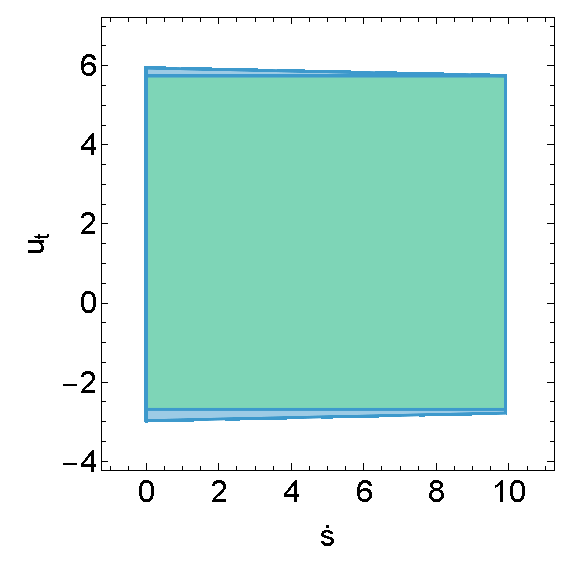
\includegraphics[width=\textwidth]{figures/inner_polytope/region_x3u1_plot_gr1.eps}
		\caption{Projection onto $\dot{s}$-$u_t$ plane}
	\end{subfigure}
	\begin{subfigure}[b]{0.32\textwidth}
		\centering
		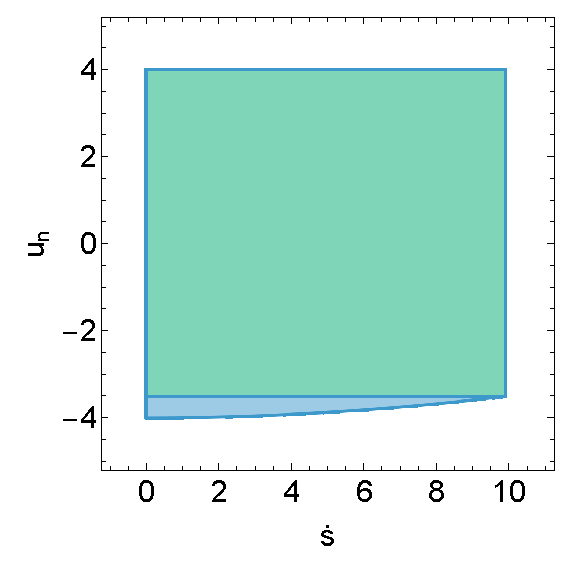
\includegraphics[width=\textwidth]{figures/inner_polytope/region_x3u2_plot_gr1.eps}
		\caption{Projection onto $\dot{s}$-$u_n$ plane}
	\end{subfigure}
	\begin{subfigure}[b]{0.32\textwidth}
		\centering
		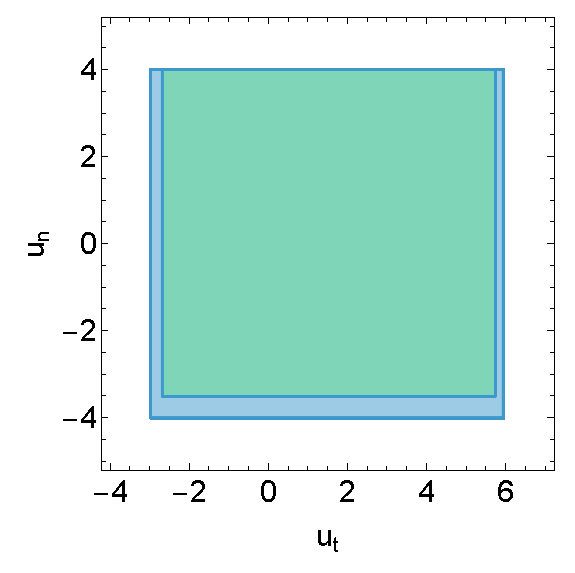
\includegraphics[width=\textwidth]{figures/inner_polytope/region_u1u2_plot_gr1.eps}
		\caption{Projection onto $u_t$-$u_n$ plane}
	\end{subfigure}
	\caption{In Green using Interval Fitting \ref{subsubsec:interval_fitting} and in Blue using CAD \ref{subsubsec:cad}.}
	\textbf{Parameters:} $C(s) \in \left[-\tfrac{1}{200},\, 0\right],\; s \in [0,\,10],\; n \in [0,\,2],\;$ \newline $v_x \in [0,\,10],\; v_y \in [-2,\,2],\; a_x \in [-3,\,6],\; a_y \in [-4,\,4],\;$ \newline $\dot{\psi} \in [-5,\,5],\; a_{\psi} \in [-2,\,2].$
	\label{fig:qe-comparison-with-params}
\end{figure}

Overall, while CAD can capture a more comprehensive feasible region, interval fitting (Approach~1) offers a compelling balance of computational
efficiency and practical accuracy, making it particularly well-suited for online or real-time motion planning.

\subsubsection{Limitations on Quantifier Elimination for Both Approaches}
\label{subsubsec:limitations_on_qe}

The general method of determining an inscribed polytope for Problem \ref{problem:inscribed_polytope} through quantifier elimination occurring in the
set \ref{eq:c_tilde} has certain limitations.

The approach tends to be conservative because the universal quantifier requires that all possible combinations of state variables must be feasible.
For instance, in a scenario with a long straight section immediately followed by a sharp left turn, the planner may enforce a single speed limit that
is valid for both segments, reducing maximum speed on the straight.
One way to mitigate this is by segmenting the road into smaller sections (e.g., splitting the straight from the turn) and defining distinct
constraint sets.
A higher-level switching mechanism can then determine when the vehicle transitions from one segment's constraints to the next.

Additionally, the initial intervals for $s$, $n$, and $\dot{n}$ in \eqref{eq:c_tilde} significantly impact the resulting feasible set.
To expand this set, the initial intervals for variables such as $\dot{s}$ and $\dot{n}$ can be chosen more precisely to reduce conservativeness.
We demonstrated this with a small nonlinear program (NLP) that treats the interval bounds as decision variables, guided by an objective function
(e.g., maximizing speed on straight segments).
As shown in Figure~\ref{fig:resulting_intervals_comparison}, a slight reduction in allowable longitudinal acceleration can result in a higher
feasible speed range, thus better utilizing the available road geometry.

\begin{figure}[h]
	\centering
	\begin{subfigure}[b]{0.45\textwidth}
		\centering
		\begin{align*}
			0    & \leq s \leq 10       \\
			0    & \leq n \leq 2        \\
			0    & \leq \dot{s} \leq 10 \\
			-2   & \leq \dot{n} \leq 2  \\
			-2.9 & \leq u_t \leq 5.9    \\
			-4   & \leq u_n \leq 3.75
		\end{align*}
		\caption{Initial Approach}
	\end{subfigure}
	\hfill
	\begin{subfigure}[b]{0.45\textwidth}
		\centering
		\begin{align*}
			0      & \leq s \leq 10,         \\
			0      & \leq n \leq 2,          \\
			0      & \leq \dot{s} \leq 10.05 \\
			-2     & \leq \dot{n} \leq 2     \\
			-2.899 & \leq u_t \leq 5.929     \\
			-4     & \leq u_n \leq 3.746
		\end{align*}
		\caption{Using Non-Linear Programming}
	\end{subfigure}
	\caption{Comparison of two sets of intervals for state variables and control inputs.}
	\label{fig:resulting_intervals_comparison}
\end{figure}

Overall, while these methods are highly effective for systematically constructing a feasible region under complex constraints, it is crucial to
mitigate over-conservativeness, particularly in dynamic driving scenarios where road geometry and speed limits vary significantly.

Next, we will introduce a transformation that maps the state variables and control inputs of the planning model to a steering angle, which can be
used to control a vehicle based on the equations from \cite{eilbrecht_challenges_2020}.
A similar approach is demonstrated in \cite{werling_optimal_2010}, which served as an additional inspiration.
